\documentclass{beamer}
%\usepackage{beamerthemeshadow}
\usepackage{graphicx}
\usepackage{amssymb}
\usepackage{amsmath}
\usepackage{eucal}
\usepackage{upgreek}




% special 
\usepackage{ifthen}
\usepackage{ifpdf}
\usepackage{float}
\usepackage{color}

% fonts
\usepackage{latexsym}
\usepackage{amsmath} 
\usepackage{amssymb} 
\usepackage{bm}
\usepackage{wasysym}


\ifpdf
\usepackage{graphicx}
\usepackage{epstopdf}
\else
\usepackage{graphicx}
\usepackage{epsfig}
\fi


%\usepackage[colorlinks,linkcolor=blue,bookmarks=true]{hyperref}

\renewcommand\mathfamilydefault{\rmdefault}

\graphicspath{{figures/},{../}}

\usetheme{Madrid}
\setbeamertemplate{navigation symbols}{}%remove navigation symbols

%%%%%%%%%%%%   dcohen cmds:

%%%%%%%%%%%%%%%%%%%%%%%%%%%%%%%%%%%%%%%%%%%%%%%%%%%%%%%%%%%%%%%%

% NEW 
\newcommand{\abs}[1]{\left|#1\right|}
\newcommand{\Prob}{\mbox{Prob}\,}
\newcommand{\erf}{\mbox{erf}\,}
\newcommand{\barline}[1]{#1}

% math symbols I
\newcommand{\sinc}{\mbox{sinc}}
\newcommand{\const}{\mbox{const}}
\newcommand{\trc}{\mbox{trace}}
\newcommand{\intt}{\int\!\!\!\!\int }
\newcommand{\ointt}{\int\!\!\!\!\int\!\!\!\!\!\circ\ }
\newcommand{\ar}{\mathsf r}
\newcommand{\im}{\mbox{Im}}
\newcommand{\re}{\mbox{Re}}

% math symbols II
\newcommand{\eexp}{\mbox{e}^}
\newcommand{\bra}{\left\langle}
\newcommand{\ket}{\right\rangle}

% Mass symbol
\newcommand{\mass}{\mathsf{m}} 
\newcommand{\Mass}{\mathsf{M}} 

% more math commands
\newcommand{\tbox}[1]{\mbox{\tiny #1}}
\newcommand{\bmsf}[1]{\bm{\mathsf{#1}}} 
%\newcommand{\amatrix}[1]{\matrix{#1}} 
\newcommand{\amatrix}[1]{\begin{matrix} #1 \end{matrix}} 
\newcommand{\pd}[2]{\frac{\partial #1}{\partial #2}}

% equations
\newcommand{\mylabel}[1]{\label{#1}} 
%\newcommand{\mylabel}[1]{\textcolor{blue}{[#1]}\label{#1}} 
\newcommand{\beq}{\begin{eqnarray}}
\newcommand{\eeq}{\end{eqnarray}} 
\newcommand{\be}[1]{\begin{eqnarray}\ifthenelse{#1=-1}{\nonumber}{\ifthenelse{#1=0}{}{\mylabel{e#1}}}}
\newcommand{\ee}{\end{eqnarray}} 

% arrangement
\newcommand{\drawline}{\begin{picture}(500,1)\line(1,0){500}\end{picture}}
\newcommand{\bitem}{$\bullet$ \ \ \ }
\newcommand{\Cn}[1]{\begin{center} #1 \end{center}}
\newcommand{\mpg}[2][1.0\hsize]{\begin{minipage}[b]{#1}{#2}\end{minipage}}
\newcommand{\mpgt}[2][1.0\hsize]{\begin{minipage}[t]{#1}{#2}\end{minipage}}
\newcommand{\putgraph}[2][width=0.30\hsize]{\includegraphics[#1]{#2}}

% more
%\newcommand{\Eq}[1]{Eq.\!\!~(\ref{#1})}
%\newcommand{\Fig}[1]{Fig.\!\!~\ref{#1}}  
\newcommand{\Eq}[1]{\textcolor{blue}{Eq.\!\!~(\ref{#1})}} 
\newcommand{\Fig}[1]{\textcolor{blue}{Fig.}\!\!~\ref{#1}} 
\newcommand{\hide}[1]{} %{\textcolor{red}{[hidden text]}} %{}
\newcommand{\rmrk}[1]{\textcolor{red}{#1}}


\begin{document}
\title[CM Theory Lunch]{Random matrix modelling of transport in sparse systems}  
\author{Yaron de Leeuw}
\institute{BGU}
\date{May 30, 2012} 

%%%%
\begin{frame}
 \titlepage
Advisor: Doron Cohen
\end{frame}

%%%%
%\begin{frame}
% \frametitle{Table of contents}
% \tableofcontents
%\end{frame}


%%%%%%
\begin{frame}
\frametitle{The model system}
We consider a system that is described by a rate equation
%
\[
\frac{dp_n(t)}{dt} = \sum_m w_{nm} p_m(t)
\]
with
\[
w_{nm} \ \ = \ \  w_0 \ \eexp{-\epsilon_{nm}} \ \eexp{-|x_n-x_m|/\xi}
\]
where:
\begin{itemize}
\item $\epsilon_{nm}>0$ is a random activation energy
\item $x_n$ are the locations of sites in space
\end{itemize}
The sites are spread uniformly so we have:
\[
\rho(r,\epsilon)drd\epsilon \ \ = \ \ \frac{\Omega_d \, r^{d-1}dr}{r_0^{d}} \ f(\epsilon)d\epsilon,     
\ \ \ \ \ \ \ \ \Omega_d=2,2\pi,4\pi
\]

For the "degenerate" model, $f(\epsilon) = \delta(\epsilon)$

\end{frame}


%%%%%
\begin{frame}
\frametitle{Diffusion coefficient}
The long term dynamics are characterized by the spreading, the survival probability and the spectral counting function. For diffusive systems:\vspace{16pt}
%\begin{itemize}
%\item $ S(t) = \left\langle r^2(t)\right\rangle \quad\sim\quad  (2d)Dt\ $
%\item $  \mathcal{P}(t) \sim  \frac{1}{\left({D t}\right)^{d/2}}        $
%\item $ \mathcal{N}(\lambda)  = \int^\lambda g(\lambda)d\lambda  \quad\sim\quad \left[\frac{\lambda}{D}\right]^{d/2} $
%\end{itemize}
\begin{align*}
 S(t) &= \left\langle r^2(t)\right\rangle \quad\sim\quad  (2d)Dt\ \\
 \mathcal{P}(t) &\sim  \frac{1}{\left({D t}\right)^{d/2}}        \\
 \mathcal{N}(\lambda)  &= \int^\lambda g(\lambda)d\lambda  \quad\sim\quad \left[\frac{\lambda}{D}\right]^{d/2} \\
\end{align*}
%
\end{frame}
%%%%%%%%%%5
\begin{frame}
\frametitle{Exact $1D$ results}
Let us define \textcolor{red}{$s\quad \equiv \quad \xi/r_0$}\\
For $1D$ with $s > 1$ we have diffusion with:
\begin{align*}
D \ \ &=\ \  \frac{s -1 }{s} w_0, 
\hspace{2cm} s \equiv \xi/r_0
\end{align*}
For $1D$ with $s < 1$ we have sub diffusion with:  \\ \vspace{8pt}
%
\fcolorbox{red}{white}{$S(t) \ \ \sim \ \ t^{2s/(1+s)}$}
\fcolorbox{red}{white}{$\mathcal{P}(t) \ \ \sim \ \ t^{-s/(1+s)}$}
\fcolorbox{red}{white}{$\mathcal{N}(\lambda) \ \ \sim  \ \ \lambda^{s/(1+s)}$}
%
\includegraphics[width=0.45\hsize]{ptsD_1D}
\includegraphics[width=0.45\hsize]{ptsD_2D}

\end{frame}

%%%%%%%
\begin{frame}
\frametitle{Numerical results for $2D$ vs $1D$}

\includegraphics[width=0.90\hsize]{pts_Spectral_PN}
\end{frame}

%%%%%%
\begin{frame}
\frametitle{RG predicition for $2D$}
RG analysis was carried out by Amir et al (Weizmann) based on the assumption that the modes are localized dimers.
The result reflects the distribution of distances between the sites.
\[ \mathcal{N}(\lambda) \ \ = \ \ \exp\left[ -\frac{\Omega_d}{2d} \Big(-\frac{\xi}{r_0} \ln(\lambda/2)\Big)^d \right]\]
\end{frame}

%%%%%%
\begin{frame}
\frametitle{Outline: diffusion coefficient}
We can estimate $D$ using several approches.
\begin{itemize}
\item Linear-Response : D is linear in the rates.
  \[D_{\textrm{LRT}} \quad = \quad \frac{1}{2d}\iint w(r,\epsilon)r^2\rho(r,\epsilon)d\epsilon dr\]
\item Effective-Range-Hopping: cutting off the non-percolative transitions.
%
\[
\iint_{w(r,\epsilon)>w_c} \rho(r,\epsilon)drd\epsilon \ \ = \ \ n_c, 
\ \ \ \ \ \ \ \ \ \mbox{with $n_c$ of order unity }
\]
%
Then we calculate $D$ as follows:
%
\[
D \ \ = \ \ D_{\tbox{ERH}}[{w}]  \ \ = \ \ \frac{1}{4}\iint \min\{w(r,\epsilon),w_c\} \ r^2  \ \rho(r,\epsilon) \ d\epsilon dr
\]
%
\end{itemize}

\end{frame}

%%%%%%
\begin{frame}
\frametitle{Variable Range Hopping}

%
\[
D_{\tbox{VRH}}[\bm{w}]  
\ \ < \ \ D_{\tbox{ERH}}[\bm{w}]
\ \ < \ \ D[\bm{w}]
\ \ < \ \ D_{\tbox{LRT}}[\bm{w}]
\]
%
VRH associates the range of the jump $r$ with its typical 
energy cost $\epsilon(r)$. 
%

\begin{columns}
\begin{column}{0.6\textwidth}
ERH threshold $w_c$ is defined via 

\[
\int\!\!\int_{w(r,\epsilon)>w_c} \rho(r,\epsilon)drd\epsilon \ \ = \ \ n_c
\]




VRH trade-off is along 

\[
\int_0^{\epsilon} \int_0^{r} \rho(r',\epsilon')  dr'd\epsilon' \ \ = \ \ n_c 
\]




VRH optimum is the $(r^*,\epsilon^*)$ point \\
where $w(r,\epsilon)$ is maximal along this curve. 



{VRH estimate} is \ \ $D \ \sim \ w(r^*,\epsilon^*) \times (r^*)^2$

\end{column}
\begin{column}{0.4\textwidth}
%%%%%%%%%%%%%%%%%%%%%%%%%%%%%%%%%%%%%%
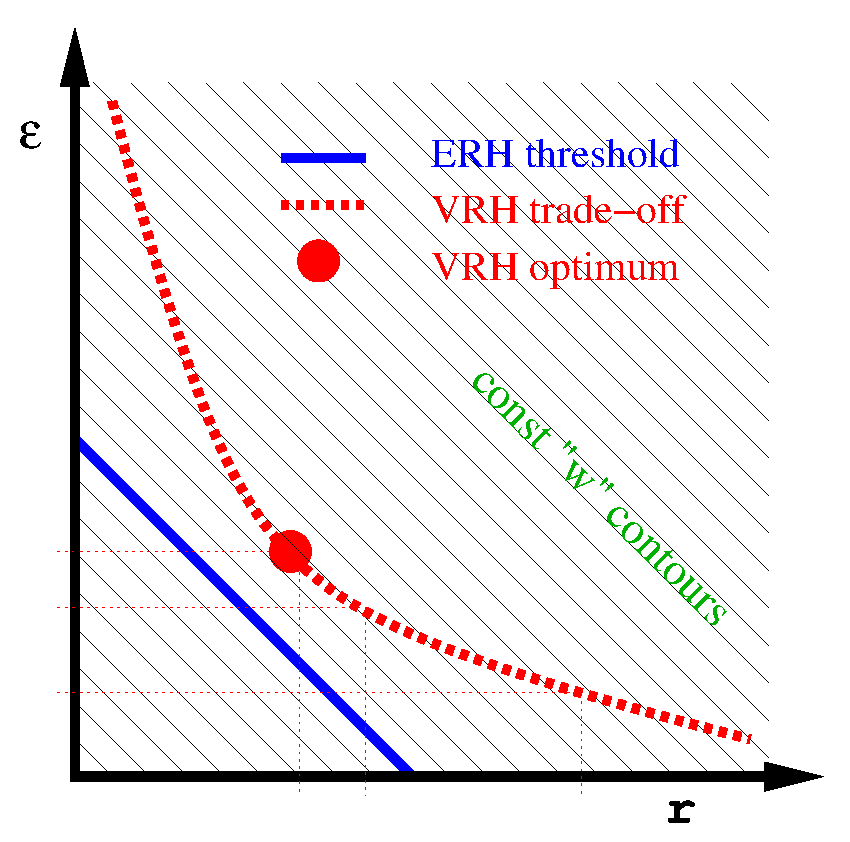
\includegraphics[width=1\hsize]{wdiagrm}
\end{column}
\end{columns}
\end{frame}

%%%%%%
\begin{frame}
\frametitle{Outline: Quasi-1D}
In the banded lattice model, the rates are:
\[  w_{nm} \ \ = \ \ w_0 \ \eexp{-\epsilon_{nm}} \ B\left(E_n-E_m\right)\]
\includegraphics[width=0.48\hsize]{ptsD_Banded_Image}
\includegraphics[width=0.48\hsize]{ptsD_Banded}\\
\includegraphics[width=0.7\hsize]{scatter_log}
\end{frame}

%%%%%%%%
\begin{frame}
\frametitle{Discussion}
%\begin{itemize}
%\item 
\begin{itemize}
  \item The localization length diverges as $\lambda$ goes to zero
  \item The density of states near $\lambda=0$ is diffusive
  \item The survival probability decays as in diffusion
  \item The spreading is diffusive
\end{itemize}
%\item  
\vspace{20pt}
Can we obtain the diffusion coefficient from the spectral properties?
%\item  

\vspace{20pt}
What should the percolation cutoff $n_c$ be?
%\end{itemize}
\end{frame}

\end{document}


